
\begin{figure}[b]%
\centering
\parbox{2.0in}{

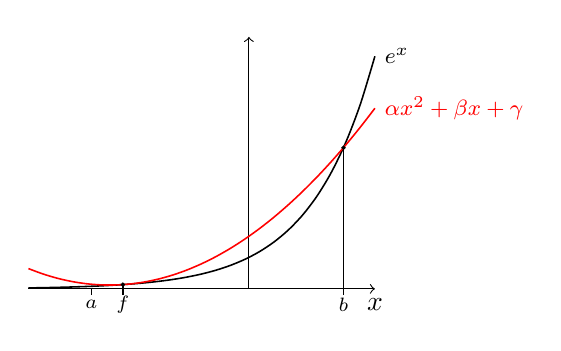
\begin{tikzpicture}[scale=0.8]
\draw[->] (-3.5,0) -- (2,0) node[anchor=north] {$x$};
\draw[->] (0,0) -- (0,4) node[anchor=east] {};
\draw[smooth, domain=-3.5:2.0, color=black, line width=0.20mm] 
    plot (\x,{e^(\x)/2}) node [right] {\footnotesize $e^x$};
\draw[smooth, domain=-3.5:2.0, color=red, line width=0.20mm] 
    plot (\x,{(0.316137167001903*\x*\x + 1.39988395124422*\x + 1.67055451771745)/2}) node [right] {\footnotesize $\alpha x^2+\beta x+\gamma$};
\draw (1.5,-0.1) -- (1.5,{e^(1.5)/2});
\draw (-2,-0.1) -- (-2,{e^(-2)/2});
\draw (-2.5,-0.1) -- (-2.5,0);
\draw[black,fill] (1.5,{e^(1.5)/2}) circle (0.25mm);
\draw[black,fill] (-2,{e^(-2)/2}) circle (0.25mm);
\draw	(-2.5,-0.25) node{{\scriptsize $a$}}
		(-2,-0.25) node{{\scriptsize $f$}}
		(1.5,-0.25) node{{\scriptsize $b$}};
\end{tikzpicture}

%\caption{A parabola over an exponential curve}%
\label{fig:graph1}}
\end{figure}
